\section{Fault detection, isolation and recovery}
\label{sec:fdir}

Following the subsystem design and software architecture, this chapter analyses which faults can occur during normal operation. Related with the preliminary failure study in \autoref{sec:preliminary_analysis}, this analysis subdivides the faults into the actuators, sensors and microcontrollers - stepper motors, potentiometers and Arduinos, respectively.

This chapter follows the fault detection, isolation and recovery (FDIR) methodology: the system must detect the faults and isolate them, to avoid mission failure. Then, the controllers perform the recovery process according to 4 FDIR levels (L0 to L3). The fault analysis follows the schematic in \autoref{fig:fault_tree}. This methodology can be found in the Arduinos' source code (in appendices \ref{appendix:master} and \ref{appendix:slave}).


\begin{figure}[H]
    \centering
    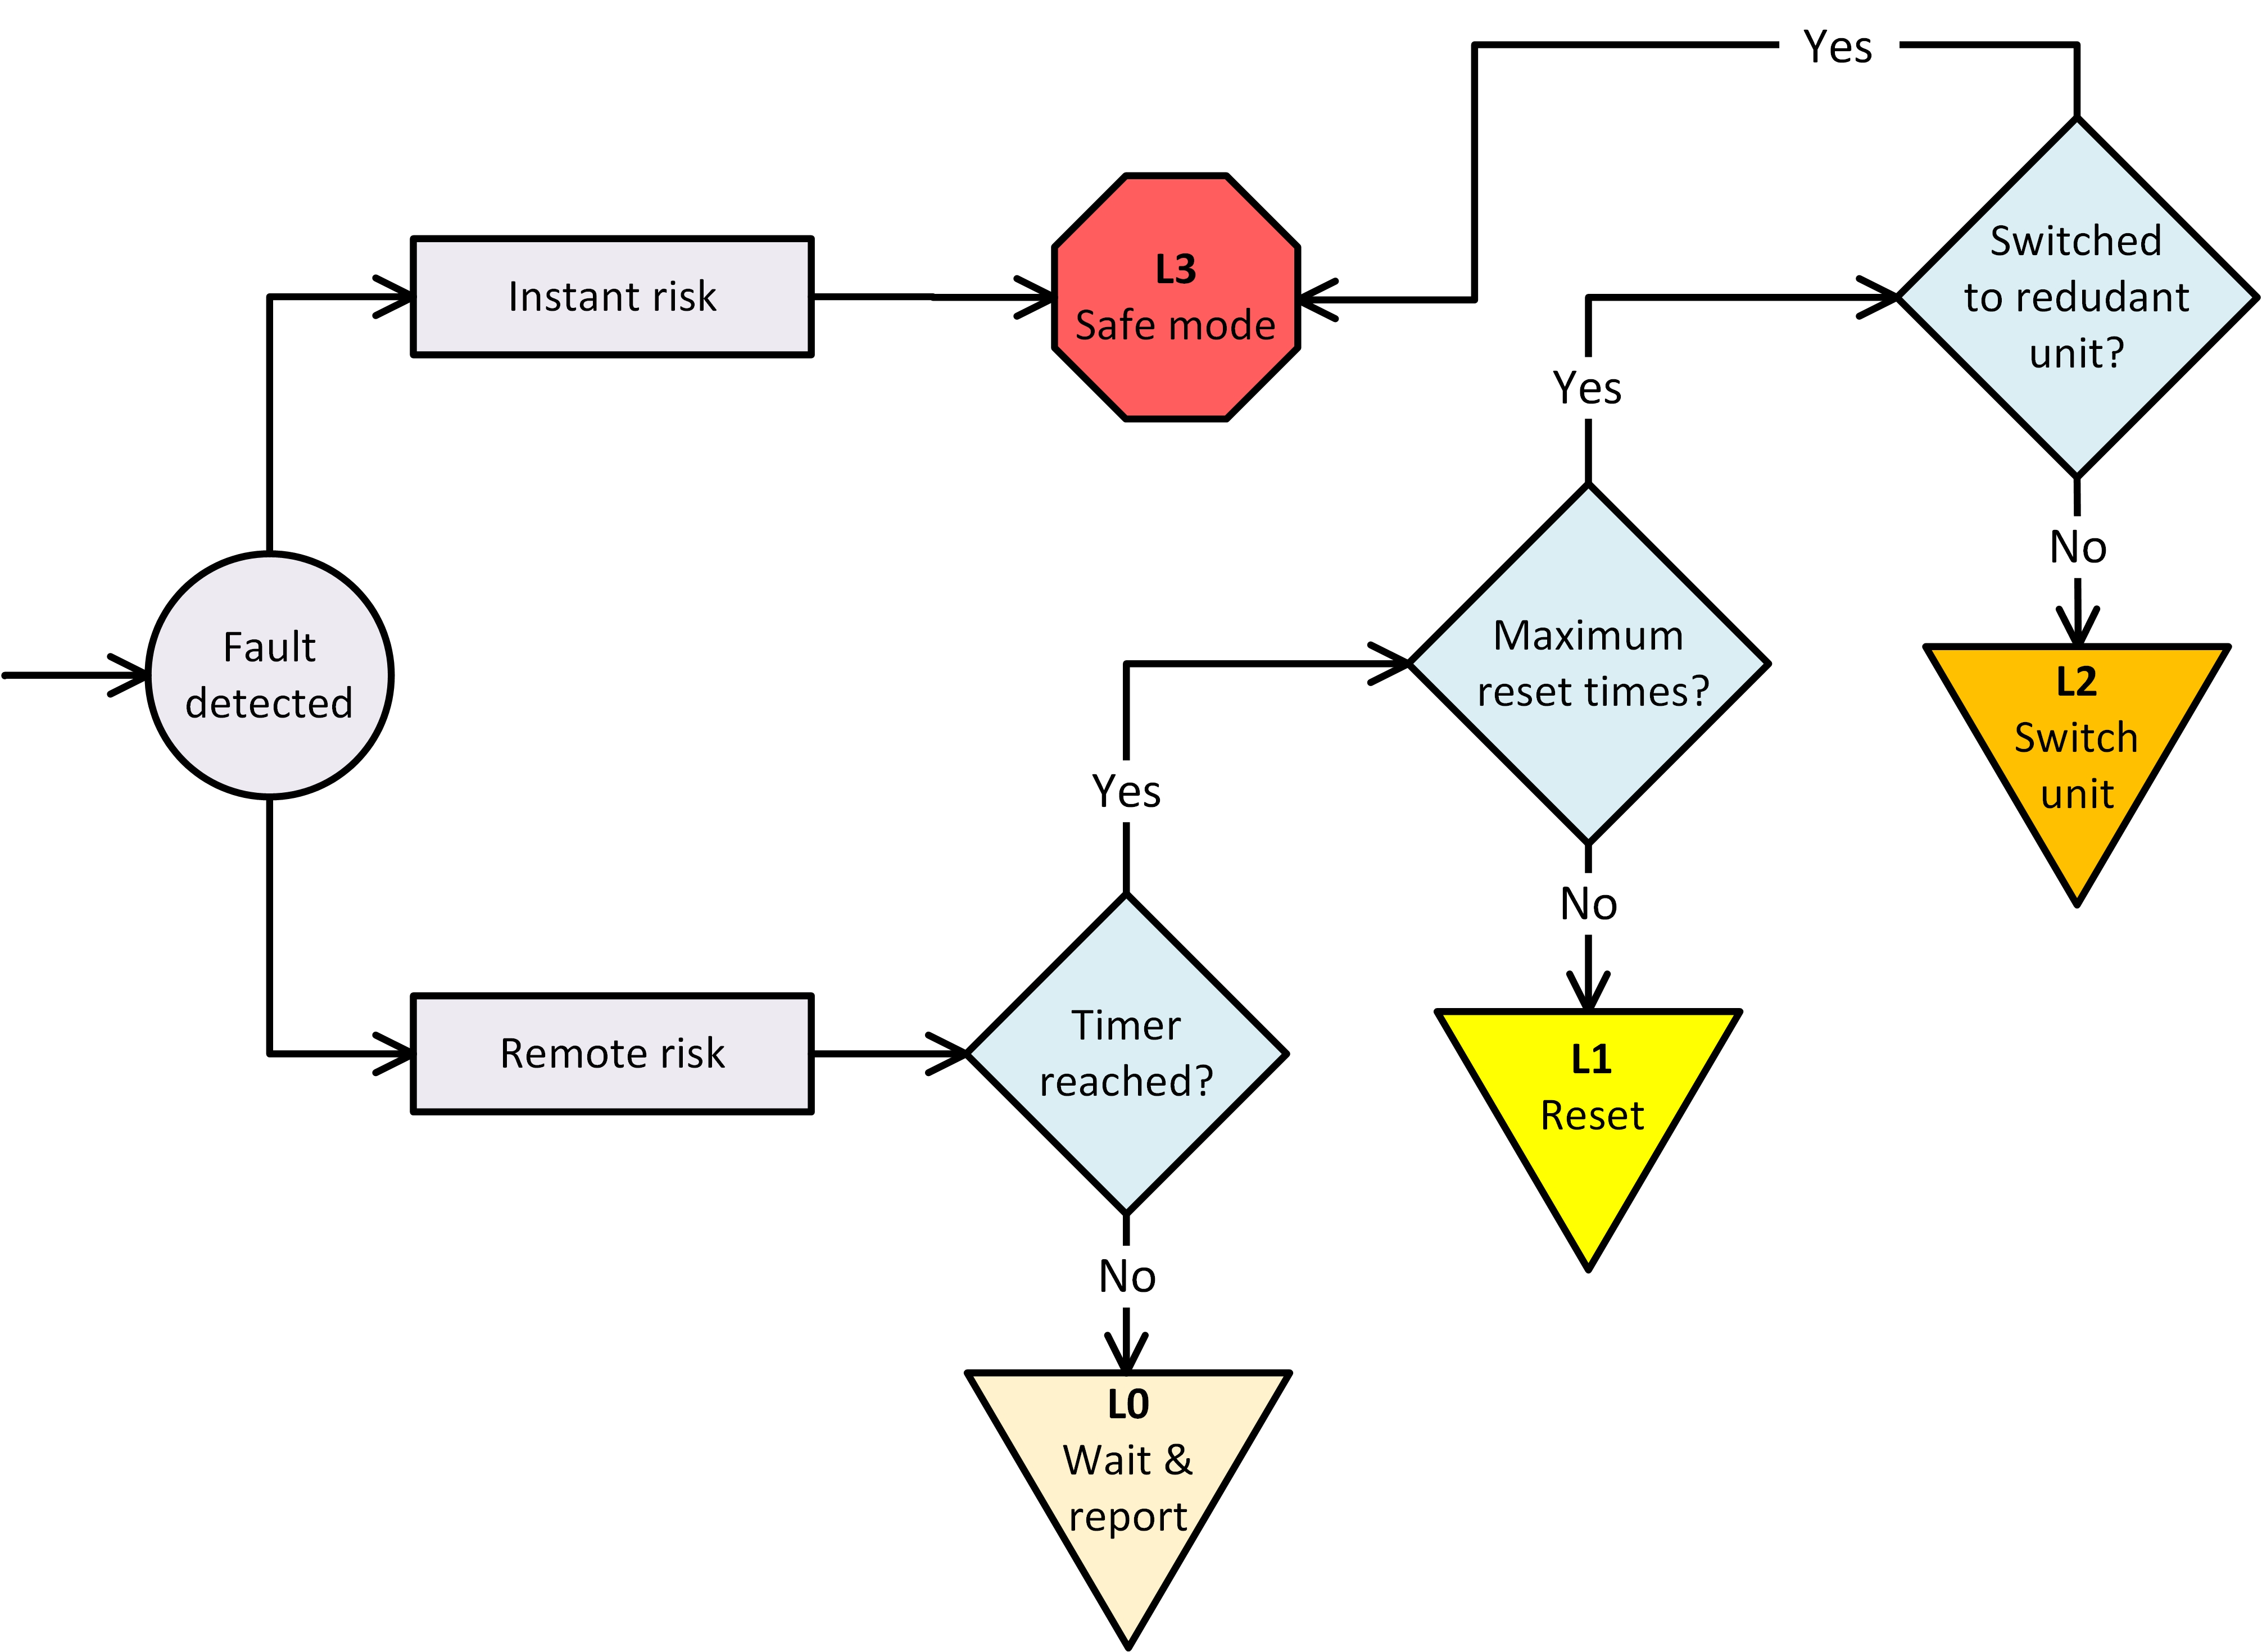
\includegraphics[width=0.8\textwidth]{figures/fdir.jpg}
    \caption{General fault recovery tree (for actuators, sensors and controllers). The timer cycle period and maximum reset times numbers are defined in \autoref{sec:fdir}.}
    \label{fig:fault_tree}
\end{figure}

Following the logic in \autoref{fig:fault_tree}, ideally, the resets (and the safe mode) can be manually or automatically triggered. Given that the communication between the computer, Arduinos and peripherals is in the order of milliseconds, the time it takes for a reset to take place is set to 5 seconds. This schematic applies entirely for the actuators and microcontrollers, while the sensors -- potentiometers -- work simultaneously and, therefore faults can only be reported (up to L0). 

The maximum reset times for the master microcontroller is one, i.e., if the slave microcontroller attempts to reset the master two times \textbf{consecutively}, the slave board takes control of the subsystem. Given the mechanical design of the mock-up, the secondary stepper motor rotates only when the sensors and primary motor disagree altogether. This option is not the ideal FDIR approach: if both stepper motors could turn the shaft (and consequently the solar panel), the controllers could implement a TBD maximum number of reset times of the primary stepper motor, after which the redundant unit would be switched on. Finally, the experimental design in \autoref{sec:experimental} cannot detect faults in the redundant units -- both the stepper motor and Arduino. Thus, the safe mode can only be manually triggered (experimentally). The ideal design would require additional units (sensors, mainly) and a more complex mechanical structure.



Faults are coded as \textit{xy}: \textit{"x"} represents the faulty component and \textit{"y"} the error number.

% communication not established, although controller 1 still working
%  -- both sending command to stepper
 
 
\subsection{Stepper motor}

\begin{table}[H]
    \centering
    \begin{tabular}{c|c|c}
        Component & ID & Description \\ \hline \hline
        \multirow{3}{*}{
            \begin{tabular}{c} Stepper\\Motor \end{tabular}}& 11 & Drift/block \\ \cline{2-3}
            & 12 & No power/No response\\ \cline{2-3}
            & 13 & No feedback \\ \hline
    \end{tabular}
    \caption{Stepper motor faults}
    \label{tab:stepper_faults}
\end{table}


\paragraph{Drift/block\\}

This fault occurs when the stepper motor rotates more (or less) than what it needs, to match the user input. It is most likely to occur with a higher number of solar panel movements, as mechanical imperfections, fluctuations in power input and low torque may affect the rotation.

Sensors, such as potentiometers, can be used to \textbf{detect} this fault. The feedback from one (or more) potentiometers, along with the motor's step information, with an appropriate voting system, provides the microcontrollers sufficient data to acknowledge the stepper's approximate true position. Thus, when the stepper drifts more than a predefined margin (or even when it blocks), the voting system can choose which angle is the actual true position. Following the tree in \autoref{fig:fault_tree}, the microcontroller resets the stepper's position. This method consists of a triple modular passive redundancy since it uses three inputs and (software) voter.

Theoretically, after a TBD number of reset times, the redundant unit should be activated (hot standby). However, due to the mock-up physical limitations, if the voter cannot determine the panel's true position, the redundant unit is activated (L2), since it is assumed that the initial stepper cannot operate the panel properly.

\textbf{Isolation} consists of detecting if both sensors acknowledge the drift/block. If the sensors are deemed to be operating correctly, then the fault 11 is correctly isolated. Otherwise, the controllers must perform a deeper sensor analysis.

In this case, if the stepper drifts and both potentiometers agree on this, L0 is skipped: the system resets the stepper's angle electronically. If an imminent crash may occur, safe mode can be manually activated. Once again, if the operator detects that the secondary stepper motor is incorrectly operating, safe-mode can also be activated (L3).




\paragraph{No power/No response\\}

If the subsystem fails to provide energy to the stepper, the motor cannot move. This fault is a sub-type of fault 11 since the stepper's response will be experimentally equal. In case that the motor does not react to the user's input, the panel's sensors (potentiometers) can detect this faulty operation. Given that the Arduino computes the stepper motor's instant step electronically, the microcontroller can assume an instant step increase/decrease with time even if the stepper blocks. Therefore, the software can only rely on the sensors to detect and isolate faults 11 and 12.

Thus, the FDIR approach, in this case, is similar to fault 11.



\paragraph{No feedback\\}

 












\subsection{Potentiometer}
















\begin{table}[H]
    \centering
    \begin{tabular}{c|c|c}
        Component & ID & Description \\ \hline \hline
        \multirow{4}{*}{Potentiometer} & 21 & No feedback \\ \cline{2-3}
            & 22 & Potentiometers disagree with each other\\ \cline{2-3}
            & 23 & Potentiometers disagree with stepper motor \\ \cline{2-3}
            & 24 & Feedback is not constant \\\hline
    \end{tabular}
    \caption{Potentiometers faults}
    \label{tab:pot_faults}
\end{table}

potentiometers are already protected to not go out of bounds from the start;

\subsection{Microcontroller}

\begin{table}[H]
    \centering
    \begin{tabular}{c|c|c}
        Component & ID & Description \\ \hline \hline
        \multirow{3}{*}{Microcontroller} & 31 & No power/No connection \\ \cline{2-3}
            & 32 & No communication between Arduinos\\ \cline{2-3}
            & 33 & No response to input \\ \hline
    \end{tabular}
    \caption{Microcontrollers faults}
    \label{tab:microcontroller_faults}
\end{table}